\section{Цель работы}

\begin{enumerate}
	\item Изучить лучшие практики по развертыванию SSL/TLS
	\item Изучить основные уязвимости и атаки на SSL последнего времени - POODLE, HeartBleed
\end{enumerate}

\section{Пример правильно настроенного сервера}

Возьмем некий сайт h31.ishere.ru. На этом сервере запущен веб-сервер nginx версии 1.4.6 с последними обновлениями безопасности.

Настройки веб-сервера, касаюшиеся TLS:

\begin{lstlisting}
listen 80;
listen 443 ssl;

ssl_certificate chain.pem;
ssl_certificate_key key.pem;

ssl_protocols TLSv1 TLSv1.1 TLSv1.2;
ssl_prefer_server_ciphers on;
ssl_ciphers 'ECDHE-RSA-AES128-GCM-SHA256:ECDHE-ECDSA-AES128-GCM-SHA256:ECDHE-RSA-AES256-GCM-SHA384:ECDHE-ECDSA-AES256-GCM-SHA384:DHE-RSA-AES128-GCM-SHA256:DHE-DSS-AES128-GCM-SHA256:kEDH+AESGCM:ECDHE-RSA-AES128-SHA256:ECDHE-ECDSA-AES128-SHA256:ECDHE-RSA-AES128-SHA:ECDHE-ECDSA-AES128-SHA:ECDHE-RSA-AES256-SHA384:ECDHE-ECDSA-AES256-SHA384:ECDHE-RSA-AES256-SHA:ECDHE-ECDSA-AES256-SHA:DHE-RSA-AES128-SHA256:DHE-RSA-AES128-SHA:DHE-DSS-AES128-SHA256:DHE-RSA-AES256-SHA256:DHE-DSS-AES256-SHA:DHE-RSA-AES256-SHA:!aNULL:!eNULL:!EXPORT:!DES:!RC4:!3DES:!MD5:!PSK';
ssl_session_cache shared:SSL:10m;
ssl_dhparam dhparam.pem;
ssl_stapling on;
ssl_stapling_verify on;
ssl_trusted_certificate chain.pem;
\end{lstlisting}

Просканируем сервер с помощью SSL Server Test:

\begin{figure}[H]
	\centering
	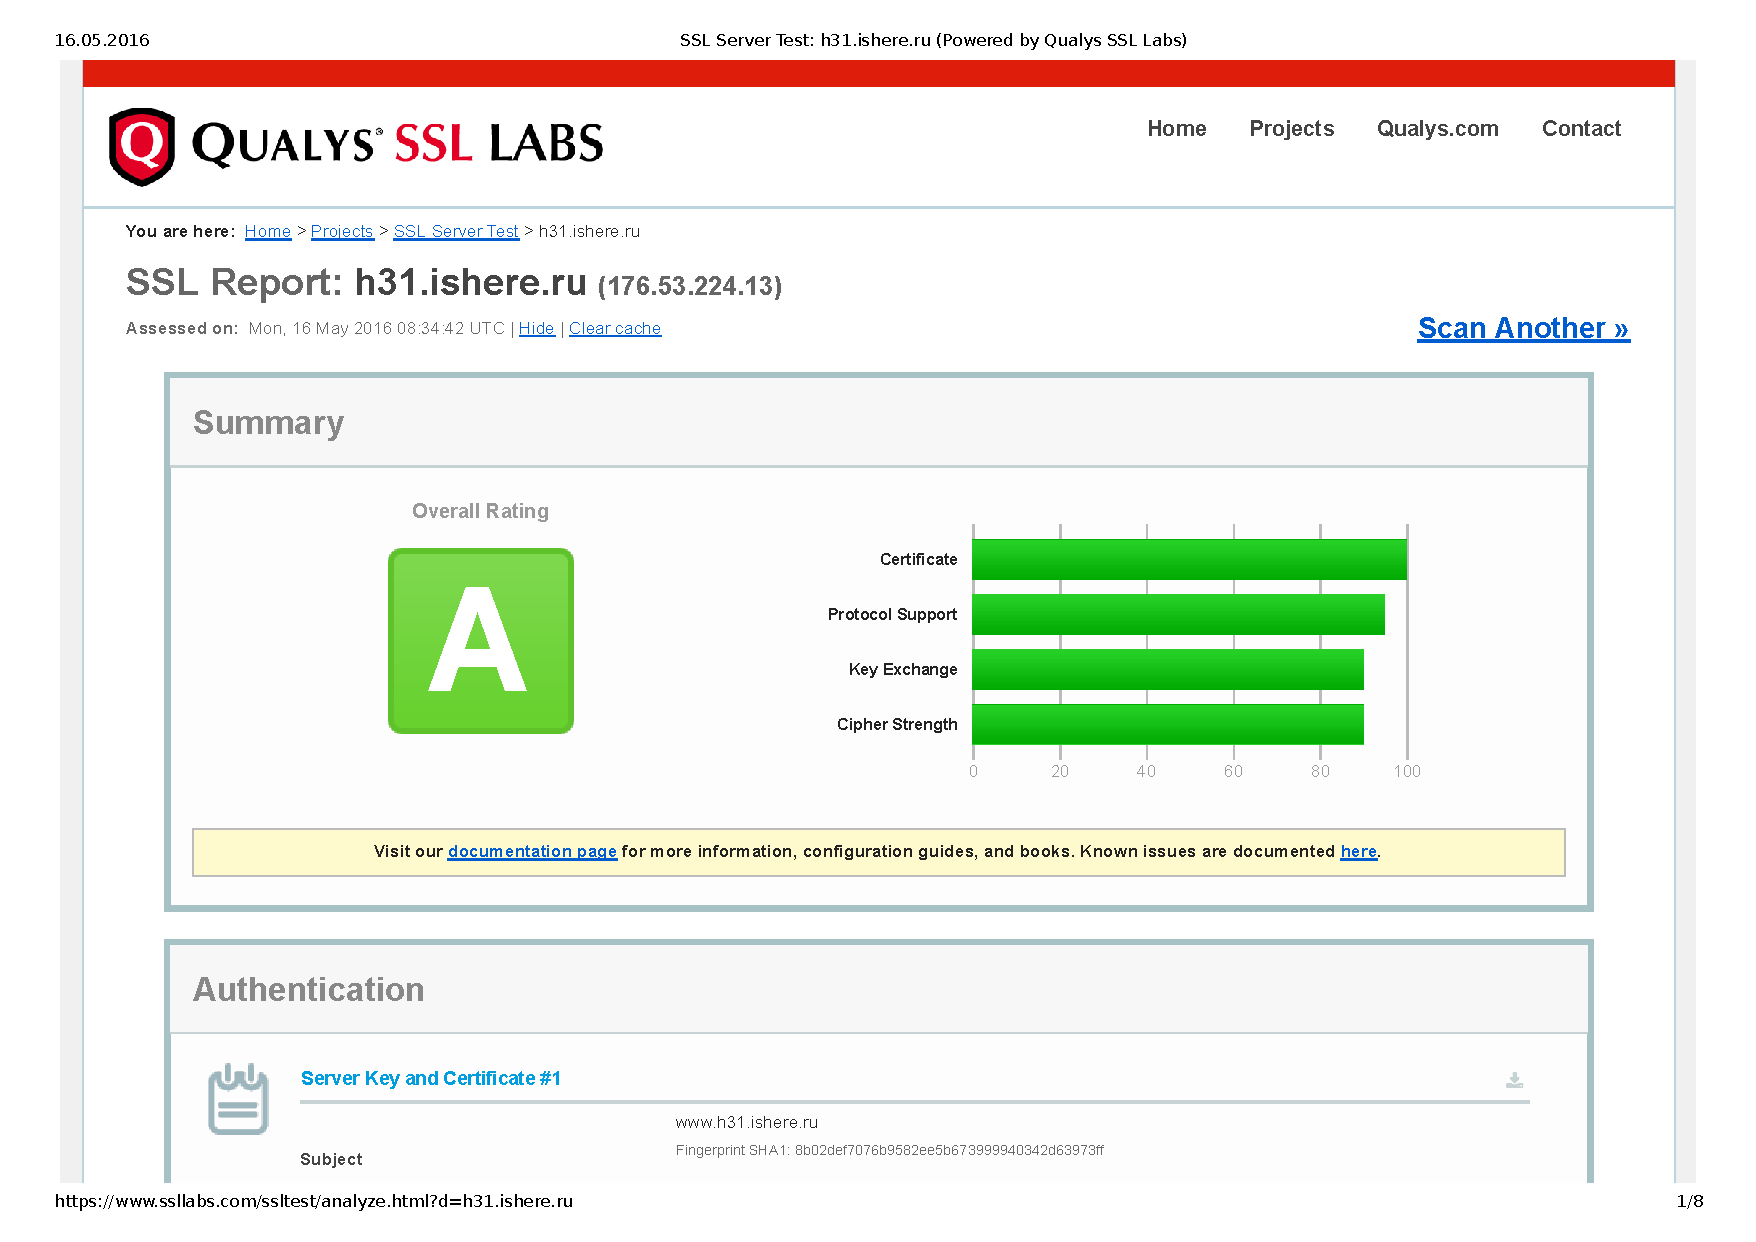
\includegraphics[width=\textwidth]{test1.pdf}
	\caption{Отчет SSL Server Test для h31.ishere.ru}
\end{figure}

В логах веб-сервера можно увидеть обращения от сервиса:

\begin{lstlisting}
64.41.200.101 - - [16/May/2016:11:32:33 +0300] "GET / HTTP/1.0" 200 1773 "-" "SSL Labs (https://www.ssllabs.com/about/assessment.html)"
64.41.200.101 - - [16/May/2016:11:32:45 +0300] "GET /?SSL_Labs_Renegotiation_Test=User_Agent_May_Not_Show HTTP/1.0" 400 0 "-" "SSL Labs (https://www.ssllabs.com/about/assessment.html)"
64.41.200.101 - - [16/May/2016:11:32:46 +0300] "GET /?SSL_Labs_Renegotiation_Test=User_Agent_May_Not_Show HTTP/1.0" 400 0 "-" "SSL Labs (https://www.ssllabs.com/about/assessment.html)"
\end{lstlisting}

\subsection{Расшифровка аббревиатур}
\begin{itemize}
	\item TLS\_ECDHE - алгоритм Диффи-Хэлмана на эллиптических кривых;
	\item RSA - алгоритм шифрования с открытым ключем;
	\item AES\_128 - алгоритм шифрования с длиной ключа в 128 бит;
	\item GCM и CBC - режимы блочного шифрования;
	\item SHA256 - хэш-функция с длиной ключа 256 бит.
\end{itemize}

\subsection{Аутентификация}
\begin{itemize}
	\item Имя основного домена:
	\begin{lstlisting}
Subject	www.h31.ishere.ru 
Fingerprint SHA1: 8b02def7076b9582ee5b673999940342d63973ff
Pin SHA256: Ln8/YgY3VzhA229r6cuXoUd0wzD4XiUoTRzi/NLCq3I=
	\end{lstlisting}
	
	\item Сетификат ещё актуален
	\begin{lstlisting}
Valid until	Mon, 20 Jun 2016 18:28:00 UTC (expires in 1 month and 4 days)
	\end{lstlisting}
	
	\item Центр сертификации:
	\begin{lstlisting}
Issuer	Let's Encrypt Authority X1 
AIA: http://cert.int-x1.letsencrypt.org/
	\end{lstlisting}
	
	\item Способ информирования об отзыве сертификата
	\begin{lstlisting}
Revocation information	OCSP 
OCSP: http://ocsp.int-x1.letsencrypt.org/ 
	\end{lstlisting}
	
	\item Можно ли доверять сертификату
	\begin{lstlisting}
Trusted	Yes
	\end{lstlisting}
	
	\item Цепочка сертификатов
	\begin{lstlisting}
1	Sent by server	www.h31.ishere.ru 
Fingerprint SHA1: 8b02def7076b9582ee5b673999940342d63973ff
Pin SHA256: Ln8/YgY3VzhA229r6cuXoUd0wzD4XiUoTRzi/NLCq3I= 
RSA 2048 bits (e 65537)	/ SHA256withRSA
2	Sent by server	Let's Encrypt Authority X1 
Fingerprint SHA1: 3eae91937ec85d74483ff4b77b07b43e2af36bf4
Pin SHA256: YLh1dUR9y6Kja30RrAn7JKnbQG/uEtLMkBgFF2Fuihg= 
RSA 2048 bits (e 65537)	/ SHA256withRSA
3	In trust store	DST Root CA X3   Self-signed	
Fingerprint SHA1: dac9024f54d8f6df94935fb1732638ca6ad77c13
Pin SHA256: Vjs8r4z+80wjNcr1YKepWQboSIRi63WsWXhIMN+eWys= 
RSA 2048 bits (e 65537)	/ SHA1withRSA 
Weak or insecure signature, but no impact on root certificate
	\end{lstlisting}
	
\subsection{Аутентификация}
	
	\item Версии TLS. Безопасные - поддерживаются, небезопасные - отключены.
	\begin{lstlisting}
Protocols
TLS 1.2	Yes
TLS 1.1	Yes
TLS 1.0	Yes
SSL 3	No
SSL 2	No
	\end{lstlisting}
	
	\item Протоколы шифрования. Предпочитается AES-GCM с обменом ключами с помощью ECDHE.
	\begin{lstlisting}
TLS_ECDHE_RSA_WITH_AES_128_GCM_SHA256 (0xc02f)   ECDH secp256r1 (eq. 3072 bits RSA)   FS	128
TLS_ECDHE_RSA_WITH_AES_256_GCM_SHA384 (0xc030)   ECDH secp256r1 (eq. 3072 bits RSA)   FS	256
TLS_DHE_RSA_WITH_AES_128_GCM_SHA256 (0x9e)   DH 2048 bits   FS	128
TLS_DHE_RSA_WITH_AES_256_GCM_SHA384 (0x9f)   DH 2048 bits   FS	256
TLS_ECDHE_RSA_WITH_AES_128_CBC_SHA256 (0xc027)   ECDH secp256r1 (eq. 3072 bits RSA)   FS	128
TLS_ECDHE_RSA_WITH_AES_128_CBC_SHA (0xc013)   ECDH secp256r1 (eq. 3072 bits RSA)   FS	128
TLS_ECDHE_RSA_WITH_AES_256_CBC_SHA384 (0xc028)   ECDH secp256r1 (eq. 3072 bits RSA)   FS	256
TLS_ECDHE_RSA_WITH_AES_256_CBC_SHA (0xc014)   ECDH secp256r1 (eq. 3072 bits RSA)   FS	256
TLS_DHE_RSA_WITH_AES_128_CBC_SHA256 (0x67)   DH 2048 bits   FS	128
TLS_DHE_RSA_WITH_AES_128_CBC_SHA (0x33)   DH 2048 bits   FS	128
TLS_DHE_RSA_WITH_AES_256_CBC_SHA256 (0x6b)   DH 2048 bits   FS	256
TLS_DHE_RSA_WITH_AES_256_CBC_SHA (0x39)   DH 2048 bits   FS	256
	\end{lstlisting}
	
	\item Проверка основных уязвимостей. Ни одна из них не может быть применена к этому сайту.
	\begin{lstlisting}
DROWN (experimental)	No, server keys and hostname not seen elsewhere with SSLv2
(1) For a better understanding of this test, please read this longer explanation
(2) Key usage data kindly provided by the Censys network search engine; original DROWN test here
(3) Censys data is only indicative of possible key and certificate reuse; possibly out-of-date and not complete
Secure Renegotiation	Supported
Secure Client-Initiated Renegotiation	No
Insecure Client-Initiated Renegotiation	No
BEAST attack	Not mitigated server-side (more info)   TLS 1.0: 0xc013
POODLE (SSLv3)	No, SSL 3 not supported (more info)
POODLE (TLS)	No (more info)
Downgrade attack prevention	Yes, TLS_FALLBACK_SCSV supported (more info)
SSL/TLS compression	No
RC4	No
Heartbeat (extension)	Yes
Heartbleed (vulnerability)	No (more info)
OpenSSL CCS vuln. (CVE-2014-0224)	No (more info)
	\end{lstlisting}
	
	\item Forward Secrecy - при взломе сервера и получении приватного ключа не получится расшифровать старые соединения (установленные до взлома)
	\begin{lstlisting}
Forward Secrecy	Yes (with most browsers)   ROBUST (more info)
	\end{lstlisting}
\end{itemize}

Итого: сервер не уязвим к основным атакам. Можно и дальше повышать безопасность, по потеряется совместимость со старыми клиентами.

\section{Пример неправильно настроенного сервера}

Просканируем people.epfl.ch (взят из раздела Recent Worst).

\begin{figure}[H]
	\centering
	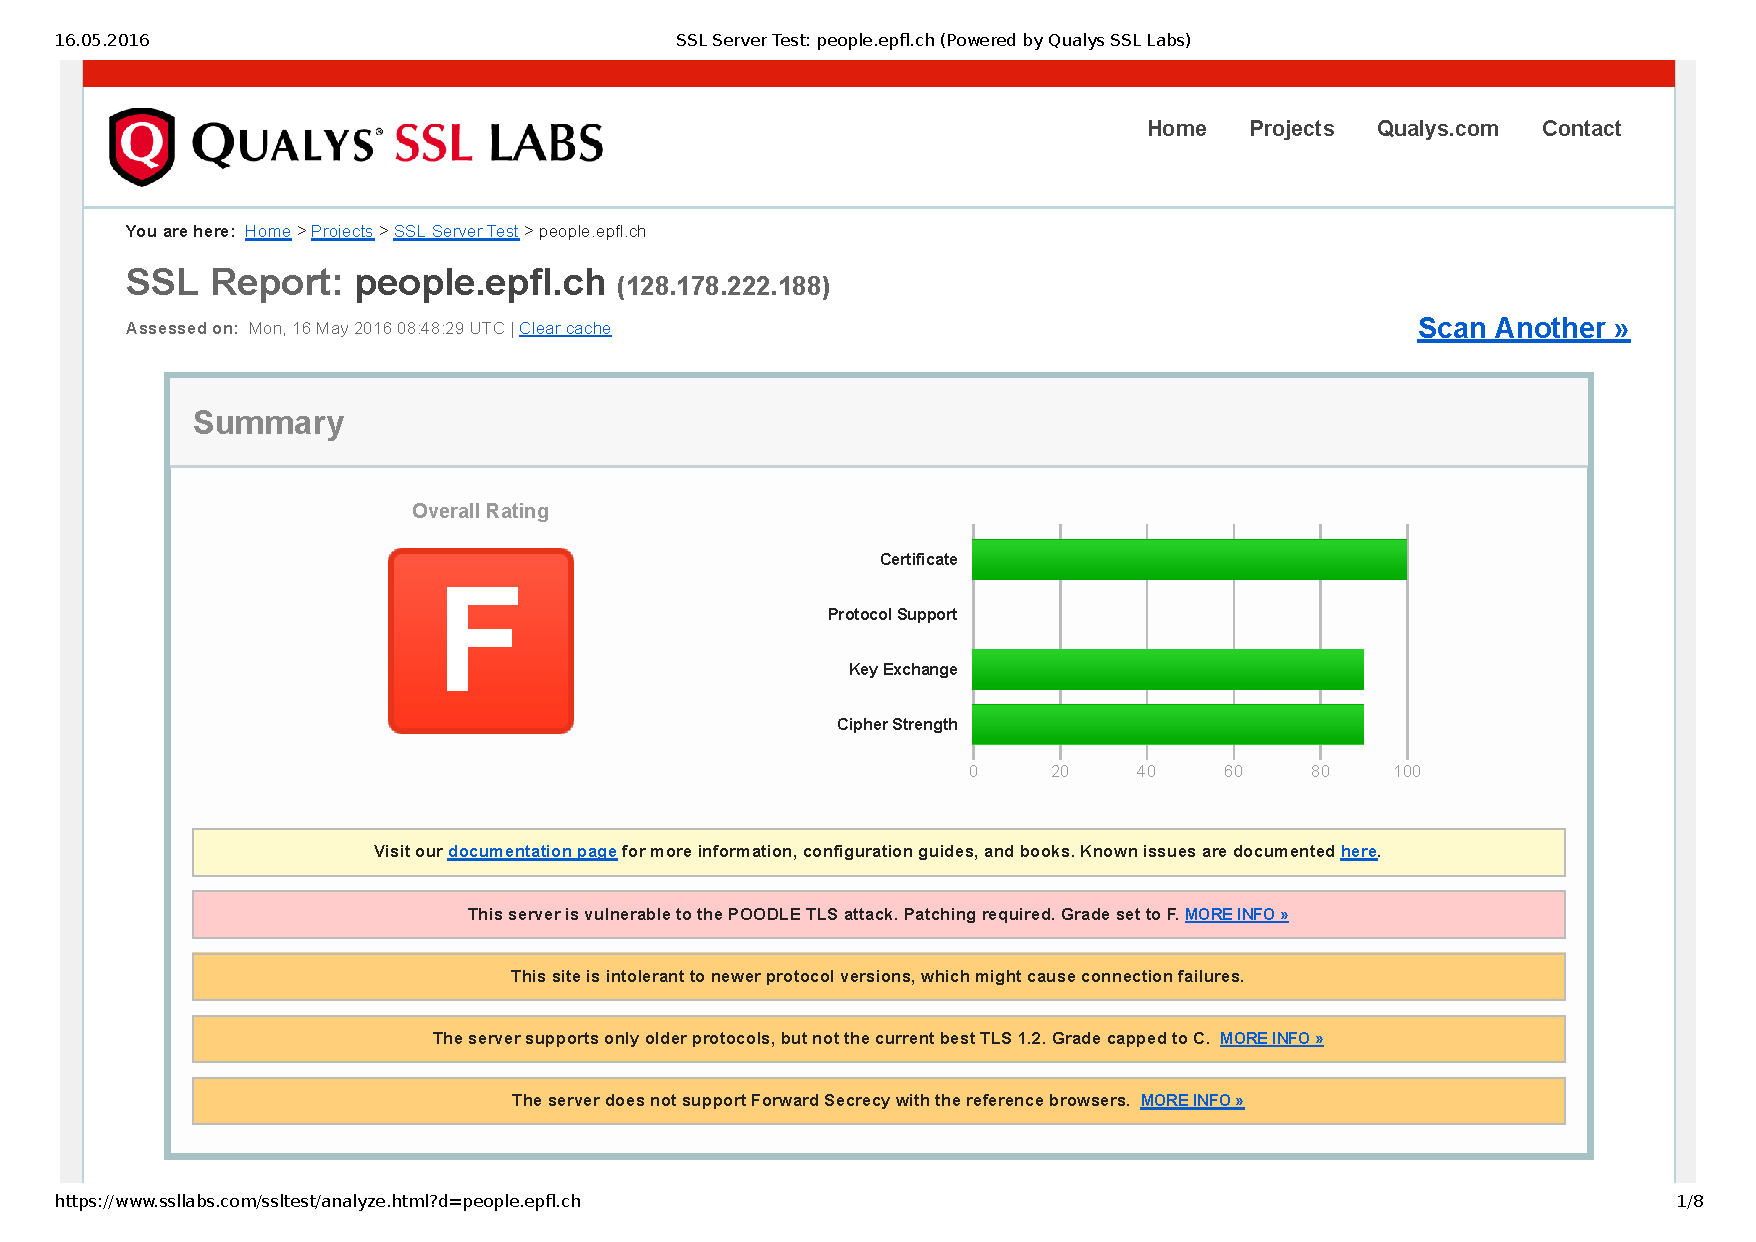
\includegraphics[width=\textwidth]{test2.pdf}
	\caption{Отчет SSL Server Test для people.epfl.ch}
\end{figure}

Этот сервер уязвим к атаке POODLE, не поддерживает Forward Secrecy и поддерживает только старые версии TLS.

\section{Пример очень хорошо настроенного сервера}

Просканируем essayoneday.com (взят из раздела Recent Best).

\begin{figure}[H]
	\centering
	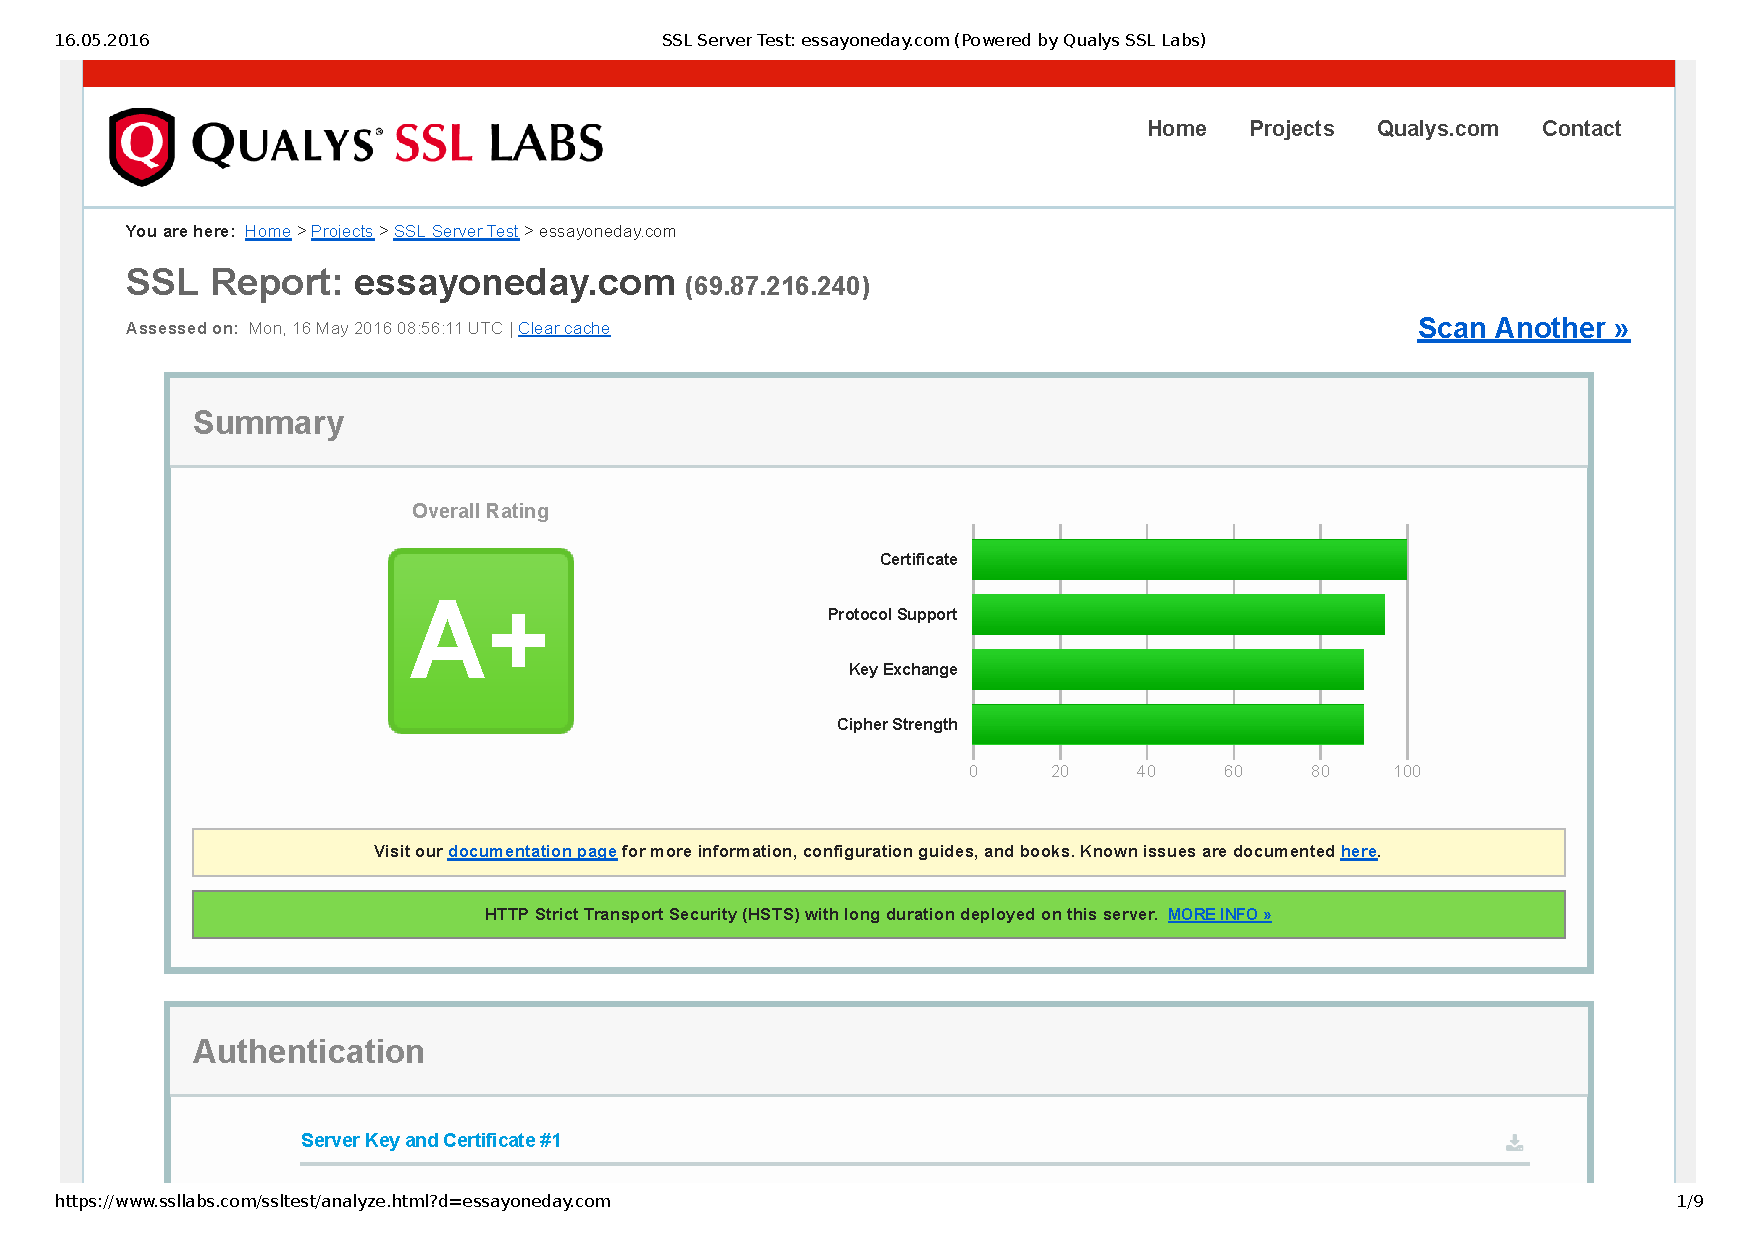
\includegraphics[width=\textwidth]{test3.pdf}
	\caption{Отчет SSL Server Test для essayoneday.com}
\end{figure}

По сравнению с первым проанализированным сайтом, добавилась поддержка HSTS. Это специальный заголовок, с помощью которого можно принудительно заставить клиента использовать только безопасное соединение (TLS) для этого сайта.

\section{Выводы}
В данной лабораторной работе был использован сервис SSL Server Test от Qualys SSL Labs. Этот сервис выдает достаточно полную информацию о поддержке SSL выбранным сервисом. Кроме того, сервис показывает основные атаки, которые могут быть применены для данного сервиса.

С помощью сервиса было проанализировано три сайта, правильно настроенного, неправильно и очень хорошо.